

\section{Desarrollo}

\subsection{Área de estudio}

Para este estudio, se utilizaron datos recolectados a partir de la utilización de ovitrampas por parte de un proyecto de la Facultad de Ingenieria de la Universidad Nacional de Entre Ríos en Oro Verde, Entre Ríos, Argentina. El área de interés se definió mediante un procesamiento en Python, utilizando las bibliotecas Folium y Pandas. Este enfoque nos permitió generar gráficos detallados que representan los puntos geográficos con información sobre la densidad de mosquitos registrada experimentalmente. En la siguiente imagen (\figurename \ref{fig:ovitrampas}), se muestra la salida de este procesamiento, con un marcador representando cada ovitrampa.
	
\begin{figure}[H]
	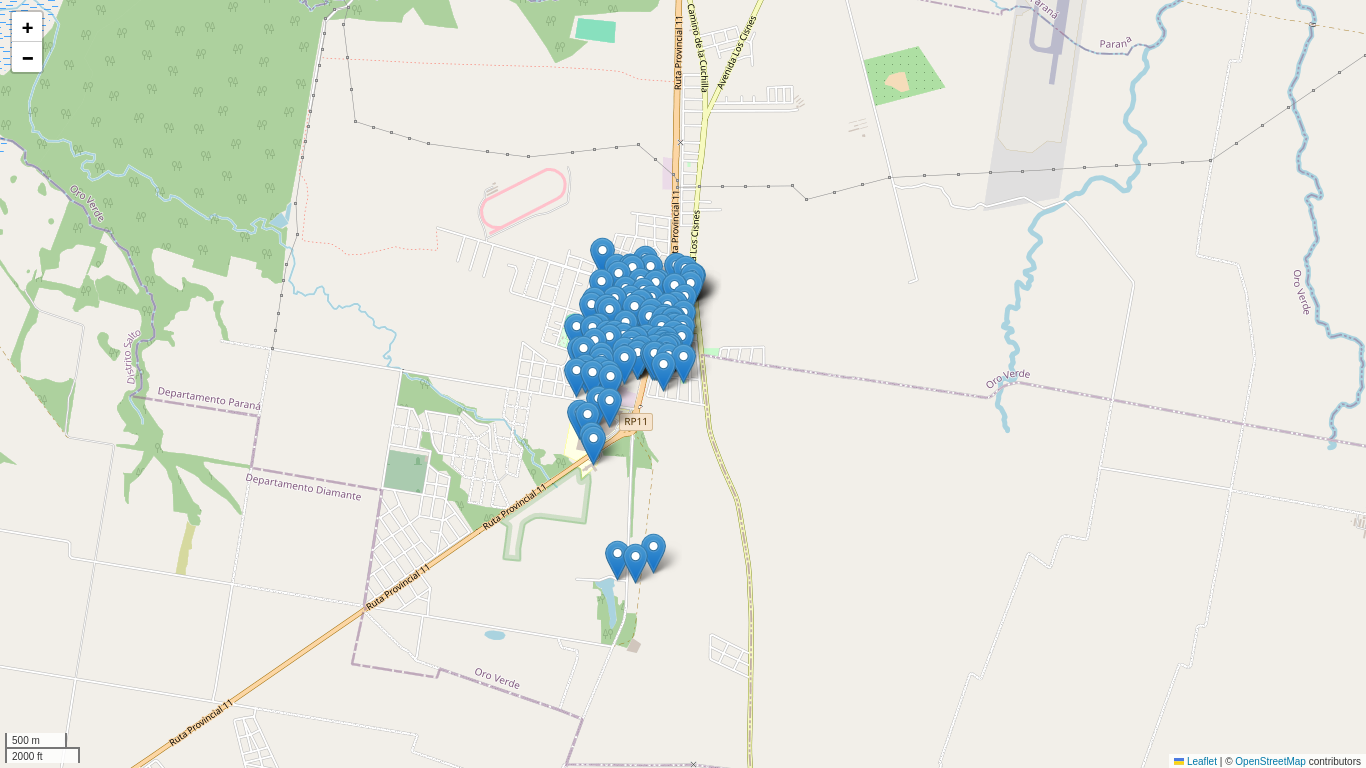
\includegraphics[width=0.7\textwidth]{ovitrampas.png}
	\centering
	\caption{Posiciones de ovitrampas en Oro Verde.}
	\label{fig:ovitrampas}
	
\end{figure}

A partir de estos marcadores, se extendió el procesamiento de los datos definiendo un cuadrado que encierra a todos los puntos con un margen adicional de 1km (\figurename \ref{fig:ovitrampas-ROI}). Esta delimitación nos permitió enfocarnos en el área específica para la cuál tenemos datos, es decir, nuestra región de interés (ROI, Region of Interest).

\begin{figure}[H]
	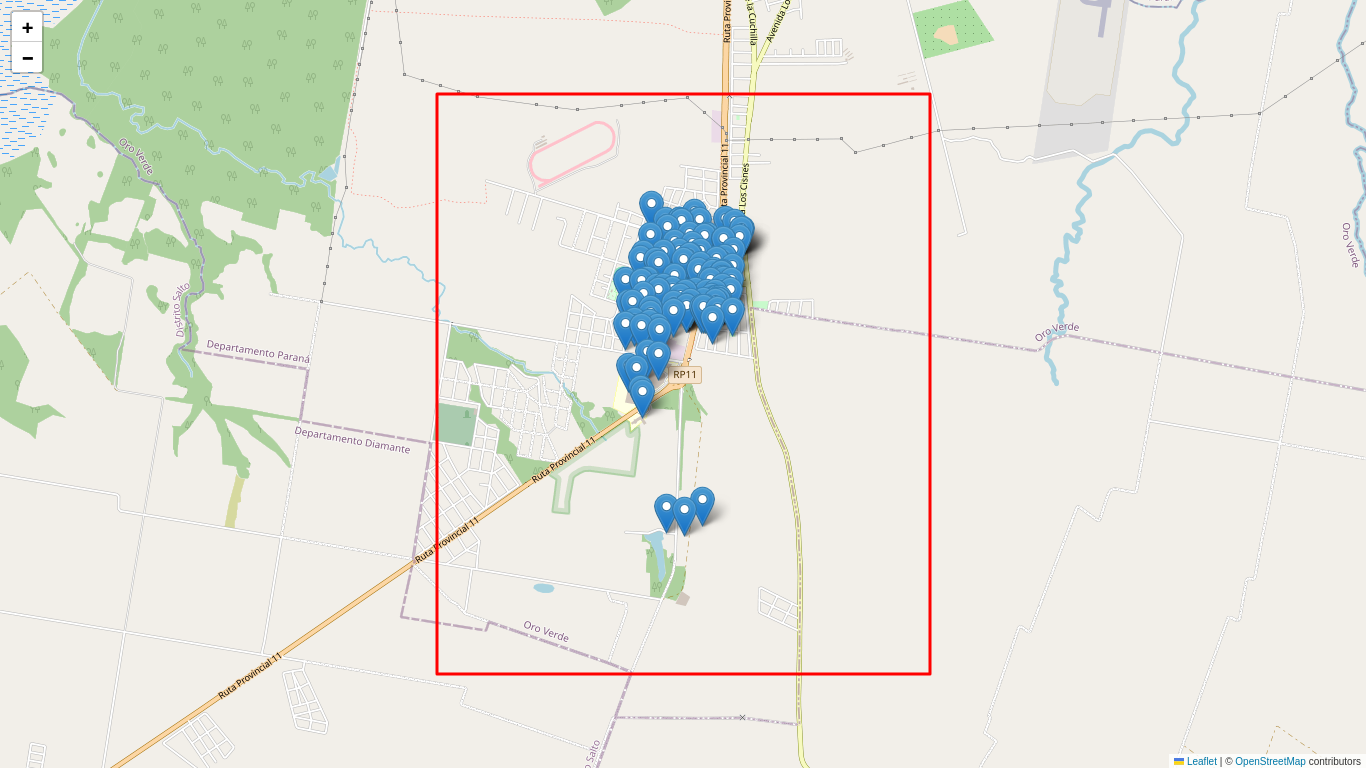
\includegraphics[width=0.7\textwidth]{ovitrampasConROI.png}
	\centering
	\caption{Posiciones de ovitrampas en Oro Verde con ROI delimitada.}
	\label{fig:ovitrampas-ROI}
	
\end{figure}

%% Podría ser buena idea agregar una foto del área de interés desde distintas perspectivas, una en la proyección mundial, otra en el mapa y después directamente la imágen.


\subsection{Obtención de imágenes}

Para el análisis, se utilizaron imágenes satelitales provenientes de Landsat 8, las cuales se obtendrán a través del Earth Explorer del USGS (United States Geological Survey) CITA. Estas imágenes, con un nivel de análisis L2, propocionan la información necesaria para estudiar la densidad de mosquitos en el área de interes a través de distintas técnicas.

\subsubsection{Dispositivo de sensado}

El Landsat 8 es un satélite de observación terreste que forma parte del Programa Landsat, administrado por el USGS y la NASA CITA. Este satelite consta de dos sensores principales:
\begin{itemize}
	\item OLI (Operational Land Imager)
	\item TIRS (Thermal Infrared Sensor)
\end{itemize}

A su vez, cada uno de estos sensores posee diversas bandas. Estas son listadas en la tabla \ref{table:landsat}.
\onehalfspacing

\begin{table}[H]
\begin{center}
	\begin{tabular}{|c | c | c|} 
		\hline
		\textbf{Banda} & \textbf{Longitud de onda ($\mu$)} & \textbf{Resolución espacial ($m$)}\\
		\hline
		1 - Coastal/Aerosol & 0.435-0.451 & 30 \\
		\hline
		2 - Azul & 0.452-0.512 & 30 \\
		\hline
		3 - Verde& 0.533-0.590 & 30 \\
		\hline
		4 - Roja & 0.636-0.673 & 30 \\
		\hline
		5 - NIR & 0.851-0.879 & 30 \\
		\hline
		6 - SWIR-1 & 1.566-1.651 & 30 \\
		\hline
		7 - SWIR-2 & 2.107-2.294 & 30 \\
		\hline
		8 - Pancromático & 0.503-0.676 & 15 \\
		\hline
		9 - Cirro & 1.363-1.384 & 30 \\
		\hline
		10 - TIR-1 & 10.60-11.19 & 100 \\
		\hline
		11 - TIR-2 & 11.50-12.51 & 100 \\
		\hline
	\end{tabular}
\end{center}
\caption{Tabla con información sobre las diferentes bandas que capta el Landsat 8}
\label{table:landsat}
\end{table}
\singlespacing

Para este estudio es muy relevante la diversidad de bandas espectrales, permitiendo analizar diversas características del terreno. Esta información, combinada con los datos de las ovitrampas, proporciona una visión integral y detallada del entorno.

%% TODO: desarrollar la comparativa con Landsat 5 que es el utilizado en el trabajo.

%% ADD PATH and ROW
\subsubsection{Análisis visual}

Como se mencionó previamente, se analizó la disponibilidad de imágenes a través de EarthExplorer. Se seleccionó la región de interés en esta plataforma y se estableció un rango de fechas según la disponibilidad de datos, comenzando con datos de  octubre de 2017. Se identificaron dos opciones de pasada del Landsat 8: una del path 227 y otra del 226, ambas para row 82. Estas opciones fueron marcadas en el mapa para evaluar la cobertura del área que proporcionaba cada una, como se muestra en \figurename \ref{fig:paths-rows}

\begin{figure}[H]
	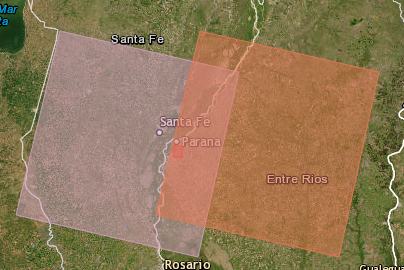
\includegraphics[width=0.7\textwidth]{pathsrows.png}
	\centering
	\caption{Opciones de cobertura.}
	\label{fig:paths-rows}
	
\end{figure}

Finalmente, se decidió utilizar la opción de la izquierda, ya que en la opción de la derecha, Oro Verde se encuentra sobre el borde de la imagen, lo que limitaría la capacidad de ampliar la región de interés. Por lo tanto, se procedió a la descarga de las imágenes correspondientes a la fecha de interés, utilizando el path 227 y el row 82.

Una vez obtenidos los datos de sensado de interés, se procedió a realizar un análisis visual detallado de la región utilizando el software QGIS. Este proceso incluyó la superposición de bandas espectrales como capas ráster y de los datos de coordenadas de las ovitrampas como vectores.

\subsection{Procesamiento de imágenes}


Con el objetivo de reducir el costo computacional y evitar el desperdicio de recursos, se procedió a definir un polígono delimitado por las coordenadas del área de interés. Este proceso incluyó la conversión de las coordenadas de las ovitrampas desde EPSG:4326 a EPSG:32620, seguido de la creación de un archivo de polígono con extensión \textit{.shp}.

Una vez que se estableció correctamente el archivo de polígono, se realizó una verificación visual utilizando QGIS para validar los cálculos (\figurename \ref{fig:polygon}). Posteriormente, se implementó el recorte de todos los archivos \textit{.TIF} utilizando la herramienta \textit{gdalwarp} de \textit{GDAL}. REFERENCIA


\begin{figure}[H]
	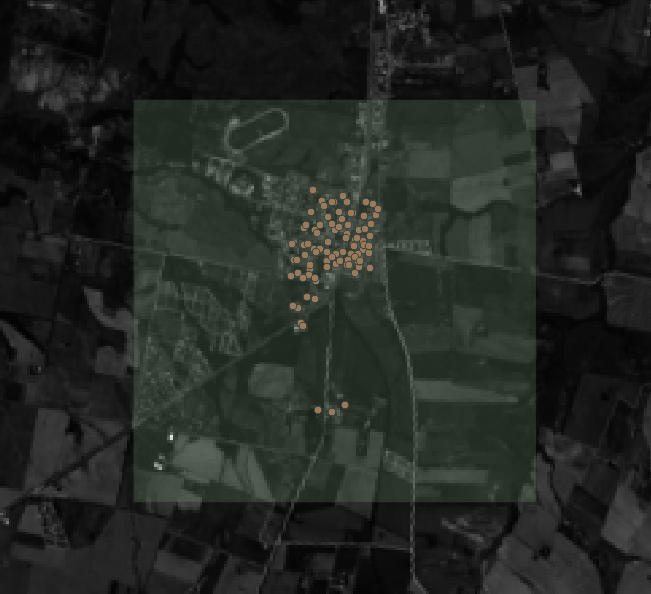
\includegraphics[width=0.7\textwidth]{polygon.png}
	\centering
	\caption{Polígono generado.}
	\label{fig:polygon}
\end{figure}

\subsection{Descripción del modelo}

$$\frac{\partial \rho(P,t)}{\partial t}=\bigtriangledown .(D_R \bigtriangledown \rho)-\bigtriangledown.(\rho D_W V)- \bigtriangledown . (\rho K_H \bigtriangledown H) + \alpha - \beta$$

Donde:

\onehalfspacing
\begin{center}
	\begin{tabular}{|c | c | c|} 
		\hline
		\textbf{Símbolo} & \textbf{Variable} & \textbf{Valor}\\
		\hline
		$$P$$ & Densidad de mosquitos & No homogéneo \\
		\hline
		$\alpha$  & Tasa de nacimientos & $6 (m^2/dia)$ \\
		\hline
		$\beta$  & Tasa de muertes             & 0.2 \\
		\hline
		$V$   & Velocidad Viento Superficie & No homogéneo \\
		\hline
		$K_H$   & Tensor de atracción         & 100 \\
		\hline
		$H$    & Campo de atracción          & No homogéneo \\
		\hline
		$D_R$   & Tensor de difusión          & No homogéneo / ver Tabla 2 \\
		\hline
		$D_W$   & Tensor de rugosidad         & No homogéneo / ver Tabla 2\\
		\hline
	\end{tabular}
\end{center}

Desglosando:

$$\frac{\partial \rho}{\partial t} (P,t)= Rozamiento(P,t)-Transporte(P,t)-Atraccion(P,t)+\alpha (P,t) - \beta (P,t¸)$$


Donde:
\doublespacing

$Rozamiento(P,t)=div[D_R (P,t) . \bigtriangledown \rho (P,t)]$

$Transporte(P,t)=[D_W (P,t) \vec{W} (P,t) . \bigtriangledown \rho (P,t)]$

$Atraccion(P,t) = div[K_H . \rho (P,t) . \bigtriangledown H (P,t)]$

\singlespacing

Con:

\begin{itemize}
	\item $\rho (P,t)$ = densidad de mosquitos
	\item $D_R (P,t)$ = tensor de rozamiento
	\item $D_W (P,t)$ = tensor de viento
	\item $W (P,t)$ = velocidad del viento
	\item $K_H$ = constante de atracción
	\item $H(P,t)$ = campo de atracción
	\item $\alpha (P,t)$ = razón de nacimientos
	\item $\beta (P,t)$ = razón de muertes
\end{itemize}


